%% GOMACTech_LaTeX.tex

\documentclass[10pt,conference]{IEEEtran}


% GOMACTech uses the standard IEEE conference format.
%
% If IEEEtran.cls, IEEEtran.bst, GOMACTech_LaTeX.bib and IEEEabrv.bib has not been installed into the LaTeX system files,
% manually specify the path to it like:
% \documentclass[conference]{../sty/IEEEtran}
%



% Some very useful LaTeX packages include:
% (uncomment the ones you want to load)

% *** COLORS ***
%\usepackage{color}
\usepackage{xcolor}% Colored text

\usepackage[most]{tcolorbox}

\usepackage{enumitem}





% *** TABLE PACKAGES **
\usepackage{multirow} % For cells that comprise more than one line of a table


% *** GRAPHICS RELATED PACKAGES ***
% \usepackage[pdftex]{graphicx}


\IEEEoverridecommandlockouts



% ***** GOMACTECH HEADER & FOOTER (IF NEEDED) *****
\makeatletter
\def\ps@IEEEtitlepagestyle{
		\def\@oddfoot{\Footer} % THIS PLACES THE FOOTER ON THE FIRST PAGE
% 	\def\@evenfoot{}
 }
\let\old@ps@headings\ps@headings
\let\old@ps@IEEEtitlepagestyle\ps@IEEEtitlepagestyle
\def\confheader#1{%
	% for all pages except the first
	\def\ps@headings{%
		\old@ps@headings%
		\def\@oddhead{\strut\hfill#1\hfill\strut}%
		\def\@evenhead{\strut\hfill#1\hfill\strut}%
		\def\@oddfoot{\Footer} % THIS PLACES THE FOOTER ON ALL PAGES AFTER THE FIRST PAGE
 }%
	% for the first page
	\def\ps@IEEEtitlepagestyle{%
		\old@ps@IEEEtitlepagestyle%
		\def\@oddhead{\strut\hfill#1\hfill\strut}%
		\def\@evenhead{\strut\hfill#1\hfill\strut}%
 }%
	\ps@headings%
}
\makeatother
% HEADER BEGINS HERE
\confheader{} % HEADER EXAMPLE 
% FOOTER BEGINS HERE
\def\Footer{
 {\footnotesize
	\begin{minipage}{\textwidth}
	\centering \scriptsize{DISTRIBUTION STATEMENT A. Approved for public release: distribution is unlimited. Approval ID: $<$XXXX-2024-XXXX$>$.\\
 }  \end{minipage}
 }
}
% ***** END GOMACTECH HEADER & FOOTER *****







% ***** DOCUMENT BEGINS HERE *****
\begin{document}



% PAPER TITLE
\title{AI Term Project Progress Report\\
 \Large{} }

% AUTHOR NAMES AND AFFILIATIONS
\author{\IEEEauthorblockN{Eric Wilson}
\IEEEauthorblockA{Advanced Radar Research Center\\
The University of Oklahoma\\
Norman, Oklahoma, United States\\
Eric.J.Wilson-1@ou.edu}\\
\and
\IEEEauthorblockN{---, ---,}
\IEEEauthorblockA{--\\
---\\
---\\
---}\\ }
\vspace{-1in}

\maketitle



\begin{abstract}
This class project aims to implement a machine learning based method of designing electrical analog filters using an unbalanced-ladder topology. The AI method developed is compared to standard filter prototypes using G-coefficients and element scaling.



%if Keywords are used, end abstract text with \\

\end{abstract}
\renewcommand\IEEEkeywordsname{Keywords}
\begin{IEEEkeywords}
AI in Analog Design, Filter Synthesis, G-coefficients, Filter prototypes, Element Scaling
\end{IEEEkeywords}



%%%%%%%%%%%%%%%%%%%%%%%%%%%%%%%%%%
%%%%%%%%%%%%%%%%%%%%%%%%%%%%%%%%%%
\section{Problem Statement}

My class presentation covered the recent developments in RF and microwave circuit design methods using AI. The basics of the RF design process were explained, and the potential for limited AI assistance at each step was briefly discussed \cite{lee2024icdesign}. Next, the distinction between parameter optimization and topological design was made. \cite{xue2023mmic} was used to demonstrate AI's ability to balance the many parameters required in an RF design whose topology is fixed. Then, the topological AI design algorithms described in \cite{xu2024microwave, karahan2024rfdesign, taskiran2024annsynthesis} were described and methods compared. Particular attention was paid to the wavelet transform used in \cite{xu2024microwave} and how it aids in inverse mapping. Additionally, the two-step learning method and fully connected layer dropout operations in \cite{karahan2024rfdesign} was discussed in depth.

My class project on the other hand involves training my own AI model which takes in circuit performance as an input (i.e. frequency vs. magnitude/phase values) and generates the circuit element values in a ladder topology to reach the desired performance. With a ladder topology circuit design (of high enough order) almost any circuit response can be generated, but choosing each circuit element's type and location in the network is complex. This is a great application of AI because it is easy to calculate the performance of a design, but difficult to determine which values are needed to achieve the circuit characteristics that are desired. The values that are determined by the AI can be compared with standard human design methods such as filter prototypes and scaling using G-coefficients.



%%%%%%%%%%%%%%%%%%%%%%%%%%%%%%%%%%
%%%%%%%%%%%%%%%%%%%%%%%%%%%%%%%%%%
\section{Background}

Understanding the standard methods designers use for filter synthesis is critical to evaluating whether using AI for filter design is actually an advantage. The basics of filter synthesis is described below.

In analog filter design the unbalanced-ladder topology for circuit design is often used. Figure~\ref{Ladder_Topology_3rd_order} shows two versions of a 3rd order ladder circuit.

\begin{figure}
	\centering
	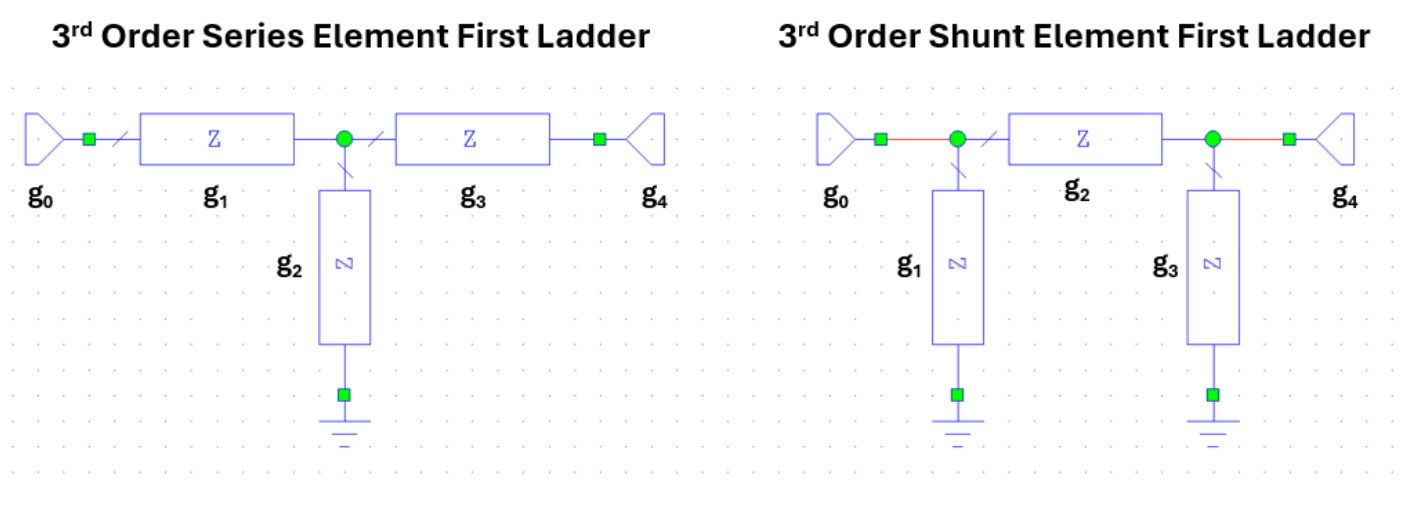
\includegraphics[width=0.9\linewidth]{Figures/Ladder_Topology_3rd_order.png}
	\caption{3rd order ladder representation: comes in series element first or shunt element first.}
	\label{Ladder_Topology_3rd_order}
\end{figure}



For standard filter synthesis there are several commonly used designs which dictate where the poles and zeros of the filter lie. Butterworth and Chebyshev filters are common and are synthesized as follows.






\textcolor{blue}{ \textbf{ --- Butterworth Filter Synthesis} }
\begin{quote}
	\begin{equation}\label{eq:gr_sine}
	g_r = 2 \sin\left( \frac{(2r - 1)\pi}{2n} \right), \quad r = 1, \ldots, n
	\end{equation}
\end{quote}

$~$
$~$


\textcolor{blue}{ \textbf{ --- Chebyshev Filter Synthesis} }
\begin{quote}

	\textcolor{blue}{ --- Insertion Loss Ripple}
	\begin{equation}\label{eq:insertion_loss}
	L_{A\_dB} = -10 \cdot \log \left( 1 - \left(10^{\frac{-L_{r\_dB}}{10}} \right) \right)
	\end{equation}

	\textcolor{blue}{ --- Ripple Factor}
	\begin{equation}\label{eq:ripple_factor}
	\epsilon = \sqrt{10^{\frac{L_{A\_dB}}{10}} - 1}
	\end{equation}

	\textcolor{blue}{ --- coefficient for input port is always 1}
	\begin{equation}\label{eq:g0}
	g_0 = 1
	\end{equation}

	\textcolor{blue}{ --- First Circuit Element }
	\begin{equation}\label{eq:g1}
	g_1 = \frac{2}{\eta} \sin\left( \frac{\pi}{2n} \right)
	\end{equation}

	\begin{equation}\label{eq:eta}
	\eta = \sinh \left[ \frac{1}{n} \sinh^{-1} \left( \frac{1}{\epsilon} \right) \right]
	\end{equation}

	\textcolor{blue}{ --- Subsequent Elements }
	\begin{equation}\label{eq:gr}
	g_r g_{r+1} = \frac{4 \sin \left( \frac{(2r - 1)\pi}{2n} \right) \sin \left( \frac{(2r + 1)\pi}{2n} \right)}{\eta^2 + \sin^2 \left( \frac{r\pi}{n} \right)}, \quad r = 1, 2, \ldots, n-1
	\end{equation}

	\textcolor{blue}{ --- Load for Odd Order Filters }
	\begin{equation}\label{eq:gload_odd}
	g_{\text{load}} = 1
	\end{equation}

	\textcolor{blue}{ \textbf{ --- Load for Even Order Filters} }
	From:

	\begin{equation}\label{eq:s21}
	|S_{21}(0)|^2 = \frac{4g_{n+1}}{(g_n + 1)^2} = \frac{1}{1 + \epsilon^2}
	\end{equation}

	Solve for \( g_{n+1} \):

	- For \( S_{11}(0) \geq 0 \):

	\begin{equation}\label{eq:gnp1_positive}
	g_{n+1} = \frac{\left( \epsilon + \sqrt{1 + \epsilon^2} \right)^2}{1}
	\end{equation}

	- For \( S_{11}(0) \leq 0 \):

	\begin{equation}\label{eq:gnp1_negative}
	g_{n+1} = \frac{1}{\left( \epsilon + \sqrt{1 + \epsilon^2} \right)^2}
	\end{equation}

\end{quote}



%%%%%%%%%%%%%%%%%%%%%%%%%%%%%%%%%%
%%%%%%%%%%%%%%%%%%%%%%%%%%%%%%%%%%
\section{Project Progress}

I wrote a program that calculates the G-coefficients for Butterworth and Chebyshev filters using the recursive equations above. I also wrote the scripts that scale those G-coefficients to get electrical component values for inductors and capacitors. Finally, I wrote a circuit simulator that has been checked against actual circuit simulator to verify accuracy. Figure~\ref{Chebyshev_G_coefs} shows the G-coefficients calculated for Chebyshev filter prototypes of different orders.


I also wrote scripts which simulates the filter circuit to measure its frequency response. The results of my circuit simulator were compared against a commercial microwave circuit simulator (Microwave Office AWR). Figure~\ref{MATLAB_vs_AWR_2} shows that my simulated filter performance exactly aligns with the commercial solver.

These scripts will be used to generate the training data and the circuit simulator will also be used to evaluate model performance.



\begin{figure}
	\centering
	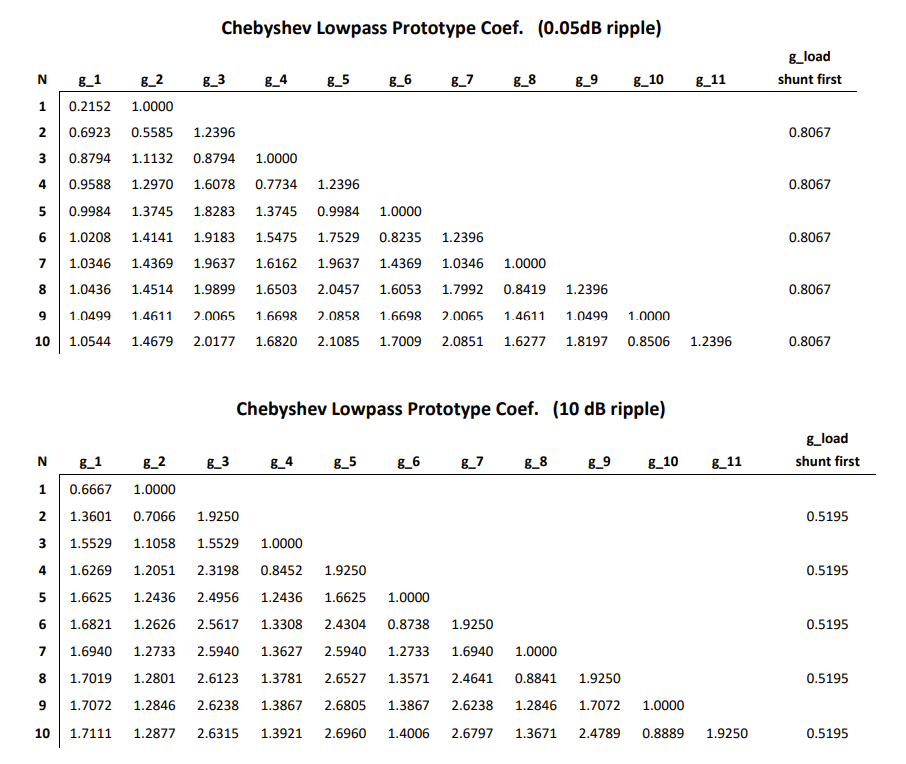
\includegraphics[width=0.9\linewidth]{Figures/Chebyshev_G_coefs.png}
	\caption{Computed Chebyshev G-coefficients. These values have been verified against other sources.}
	\label{Chebyshev_G_coefs}
\end{figure}


\begin{figure}
	\centering
	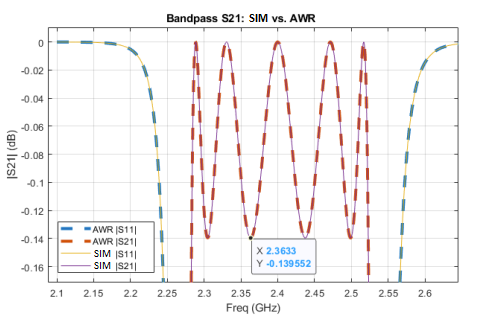
\includegraphics[width=0.9\linewidth]{Figures/MATLAB_vs_AWR_2.png}
	\caption{S21 of a bandpass filter simulated with AWR and my own script. Notice the very zoomed in vertical axis to accurately measure the filter passband ripple. My circuit simulator lines up exactly with the commercial solver.}
	\label{MATLAB_vs_AWR_2}
\end{figure}



%%%%%%%%%%%%%%%%%%%%%%%%%%%%%%%%%%
%%%%%%%%%%%%%%%%%%%%%%%%%%%%%%%%%%
\section{Project Scope}


For this project a ladder topology of 6 circuit elements is chosen over a 100x frequency bandwidth. Each circuit element has the following options: open, short, resistor, capacitor, inductor, series LC, or shunt LC. Many randomly generated circuit designs will be generated and performance calculated over the frequency range. This data will be used to train the model. The performance of the model will be based on how well it can design a circuit to match desired performance.











%%%%%%%%%%%%%%%%%%%%%%%%%%%
%%%%%%%%%%%%%%%%%%%%%%%%%%%
\section{Conclusion}
A program has been written that can calculate the G-coefficients for Butterworth and Chebyshev filters. More scripts have been written that can scale those G-coefficients to get electrical component values for inductors and capacitors. Finally, I wrote a circuit simulator that has been checked against actual circuit simulator to verify accuracy. These scripts will be used to generate the training data and the circuit simulator will also be used to evaluate model performance.





%%%%%%%%%%%%%%%%%%%%%%%%%%%
%%%%%%%%%%%%%%%%%%%%%%%%%%%
\bibliographystyle{IEEEtran}
\bibliography{citations}



% that's all folks
\end{document}